\documentclass{beamer}
\graphicspath{{images/}}
\title{ArtFinder: A Faceted Browser for Cross-Cultural Art Discovery}
\author{Matt Thompson}
\institute{University of Bath, NII Tokyo, Sysemia Ltd Bristol}
\date{}
\titlegraphic{
   
\includegraphics[width=0.6\textwidth]{uob-logo.png}
}
\usetheme{SlimRed}
\usepackage{verbatim}
\usepackage{caption}
\usepackage[caption=false]{subfig}
\usepackage{url}


\begin{document}
\frame{\titlepage}

\begin{frame}
    \frametitle{The problem}
        \begin{itemize}
            \item How to explore art from another culture?
            \item Generally, you know what you like
            \item But what if the domain is totally unknown?
        \end{itemize}
\end{frame}


\begin{frame}
    \frametitle{Datasets}
        \begin{itemize}
            \item LODAC (\url{http://lod.ac}): Japanese Artists \& Museums
            \item English DBpedia (Wikipedia articles)
            \item DBpedia Japan
            \item University of Keio's Japanese Wikipedia ontology
        \end{itemize}
\end{frame}


\begin{frame}
    \frametitle{Possible solutions}
        \begin{itemize}
            \item Search
            \item Visualisation
            \item Categorisation and browsing
        \end{itemize}
\end{frame}

\begin{frame}
    \frametitle{Search}
    \begin{figure}
        \centering
        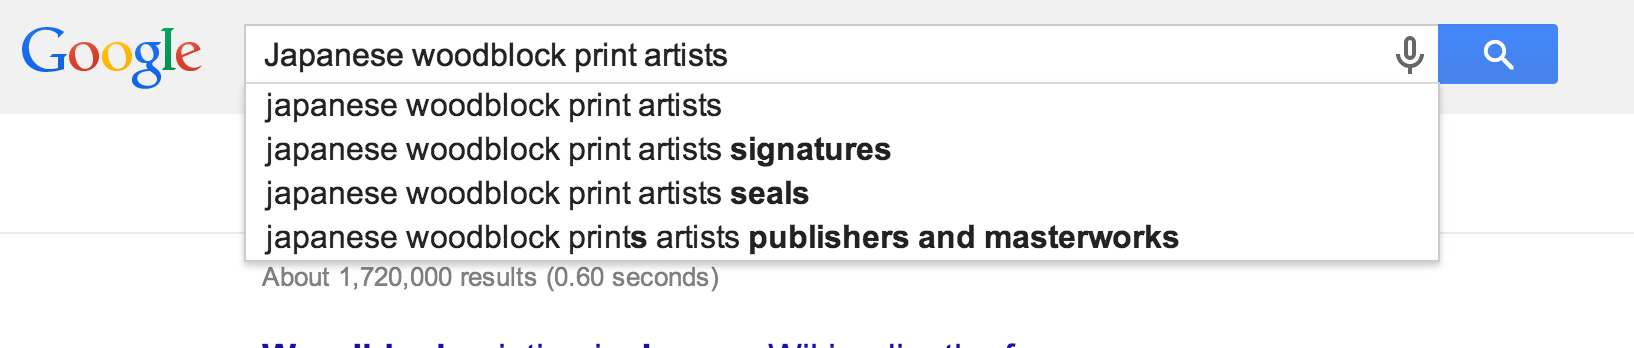
\includegraphics[width=0.9\textwidth]{search.png}
    \end{figure}
        \begin{itemize}
            \item This is the standard approach
            \item What keywords would you use?
            \item What if the genres are words in a foreign language?
        \end{itemize}
\end{frame}


\begin{frame}
    \frametitle{Visualisation}
    \begin{figure}
        \centering
        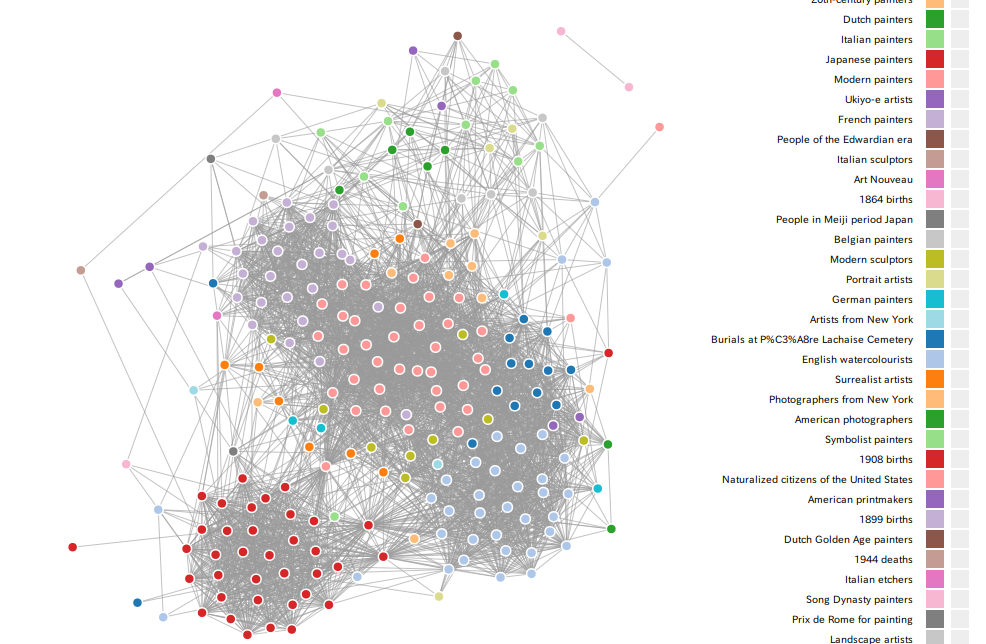
\includegraphics[width=0.6\textwidth]{artvis1.png}
    \end{figure}
        \begin{itemize}
            \item We created `ArtViz', a prototype visualisation
            \item Users can select genres of interest and `see' similar artists
            \item Could be used for genres, eras, etc
            \item Difficult to use these simultaneously, though
        \end{itemize}
\end{frame}

\begin{frame}
    \frametitle{Browsing the artists}
        \begin{itemize}
          \item One problem: browsing artists from a \emph{list} of tags is not ideal
            \item Discovering new artists is difficult for the user
            \item Ideally, the tags would be in some kind of hierarchical taxonomy
            \item How can we make this?
        \end{itemize}
\end{frame}

\begin{frame}
    \frametitle{Datasets}
    \begin{figure}
        \centering
        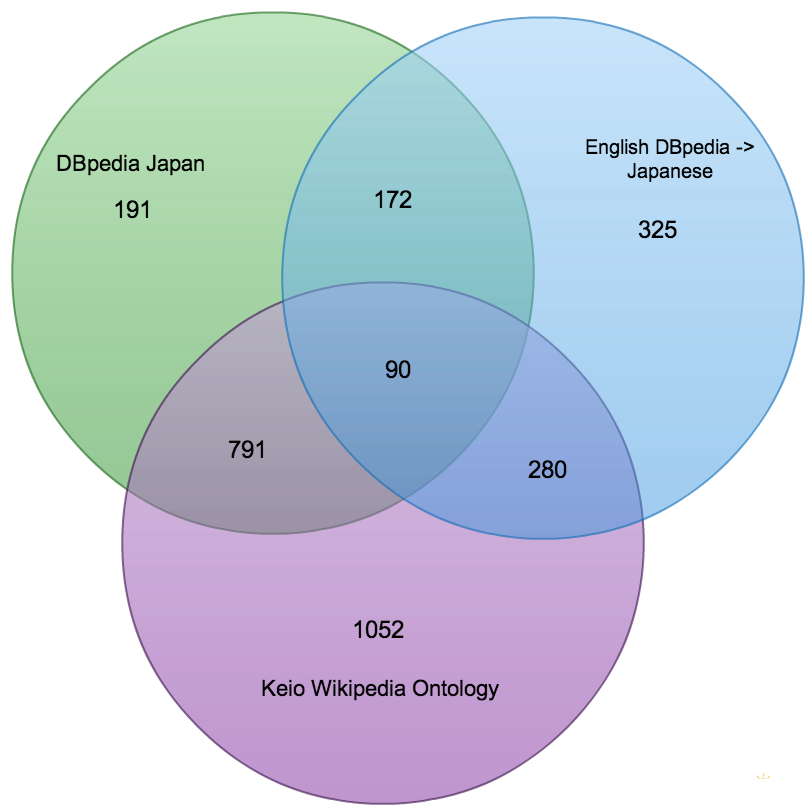
\includegraphics[width=0.5\textwidth]{venn.png}
    \end{figure}
        \begin{itemize}
            \item Cross-referenced LODAC with other ontologies
            \item Overlap (minus blanks/duplicates) of 893 usable artists
        \end{itemize}
\end{frame}

\begin{frame}
    \frametitle{Extraction and translation of tags}
        \begin{itemize}
          \item SPARQL queries sent to 893 artists
            \item Tags (genre, era, etc) taken from all ontologies
            \item Translated into English using Google Translate API
        \end{itemize}
\end{frame}

\begin{frame}
    \frametitle{Hierarchy generation}
            \[P(x|y) \geq 0.8, P(y|x) < 1, D_i > 4\]
        \begin{itemize}
            \item Used Sanderson and Croft's subsumption approach \cite{sanderson}
            \item Relaxed constraint of 0.8 gives better results
            \item Added $D_i$ (number of documents in which tag occurs) from Schmitz et al \cite{schmitz}
            \item Greedy clustering algorithm based on Heymann \cite{heymann}
        \end{itemize}
\end{frame}

\begin{frame}
    \frametitle{Faceted search}
        \begin{itemize}
            \item First devised by Ranganathan \cite{ranganathan} for library classification
            \item Sorts items into distinct, mutually exclusive facets
            \item Film example: `year', `cast', `genre'
            \item Many examples of faceted browsers, such as FLAMENCO browser for buildings \cite{hearst}
        \end{itemize}
\end{frame}

\begin{frame}
    \frametitle{Facets}
        \begin{itemize}
          \item Facets: \emph{era, location, genre, media}
            \item Determined based on Ranganathan's \cite{ranganathan} guidelines
            \item (Temporal, Spatial, Personal, Material)
        \end{itemize}
\end{frame}

\begin{frame}
    \frametitle{Browsing interface}
    \begin{figure}
        \centering
        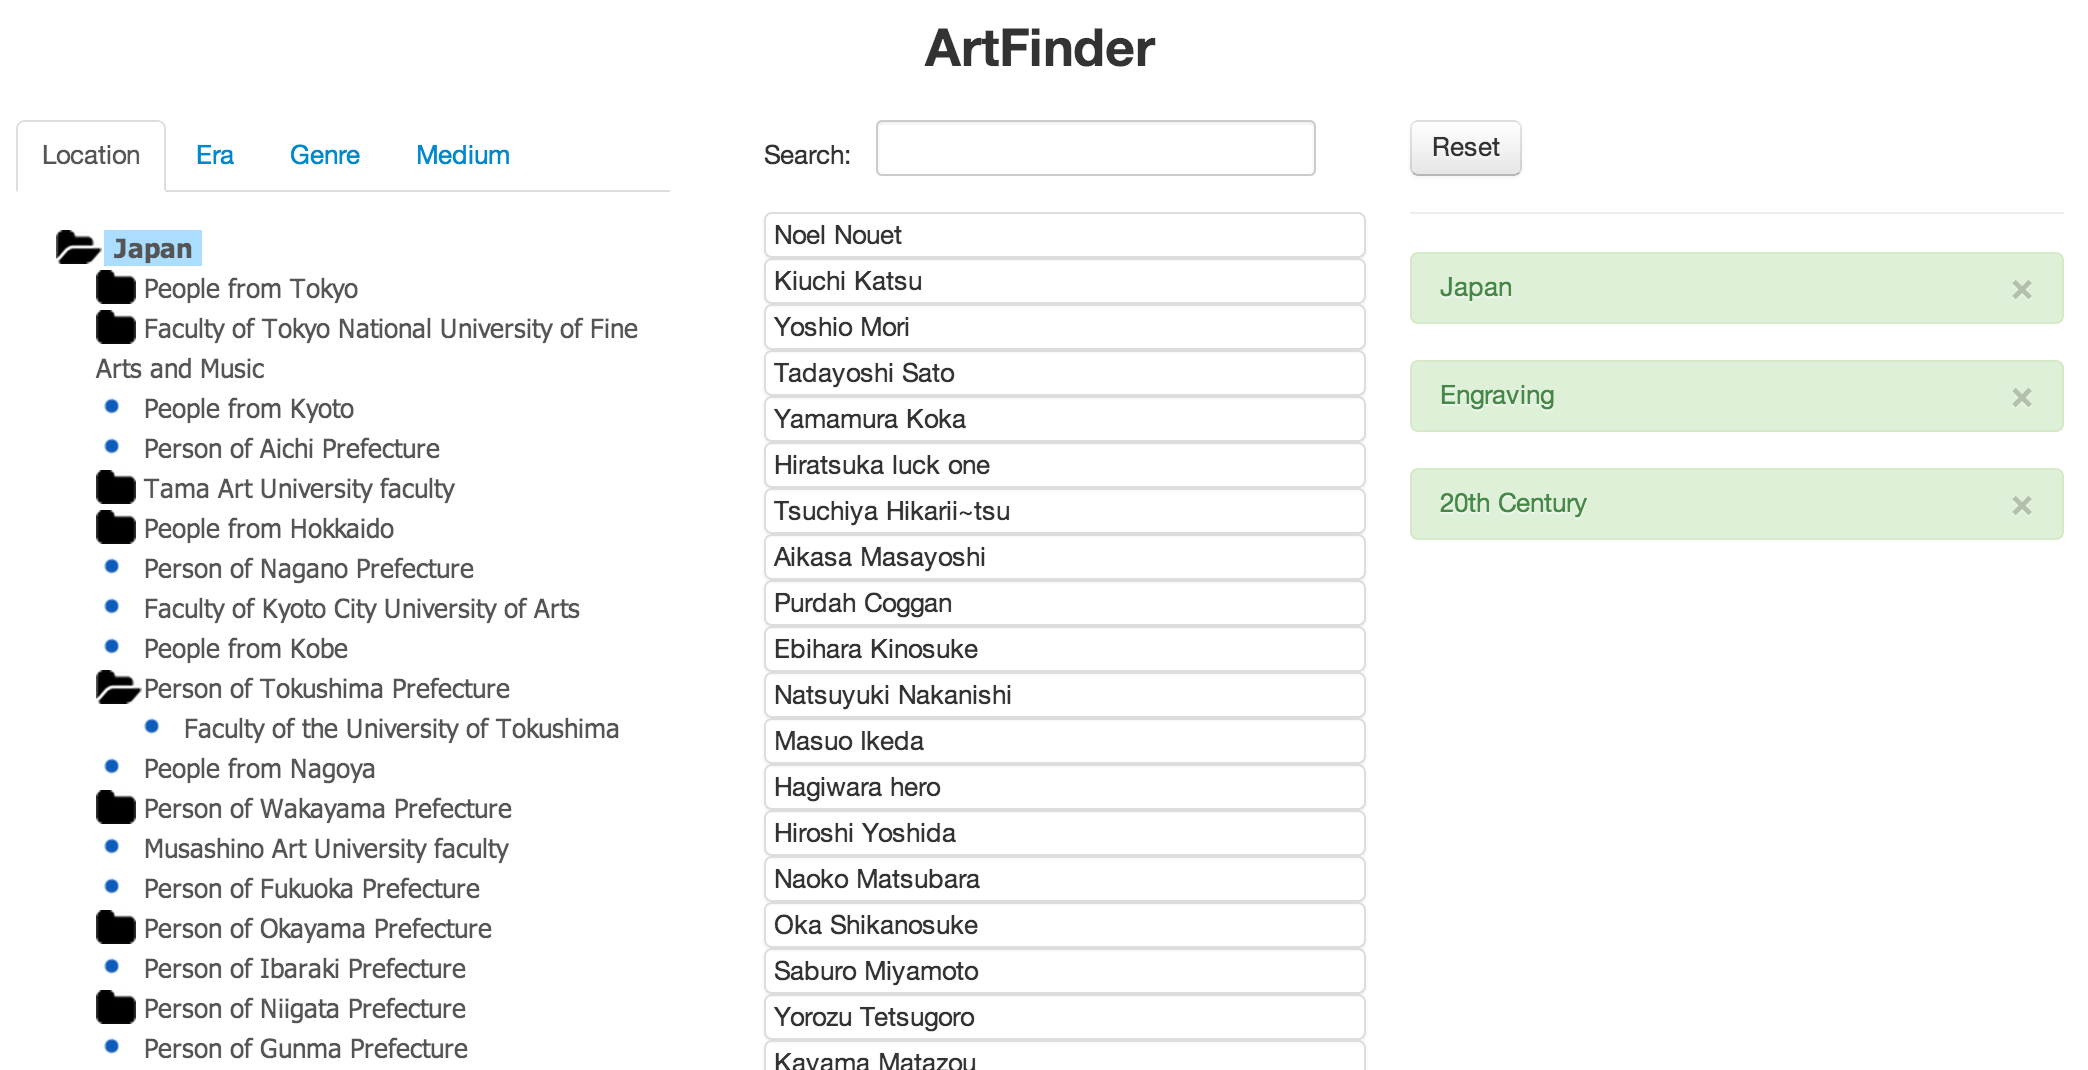
\includegraphics[width=0.7\textwidth]{artfinder1.png}
    \end{figure}
        \begin{itemize}
            \item \url{http://is.gd/artfinder}
          \item Javascript, Angular.js, JSON
            \item Multiple facets can be selected from left
        \end{itemize}
\end{frame}

\begin{frame}
    \frametitle{Preliminary user study}
\begin{figure}[!t]
  %\centering
  \subfloat[Mean time taken for each interface, by question \label{fig:results1}]{
  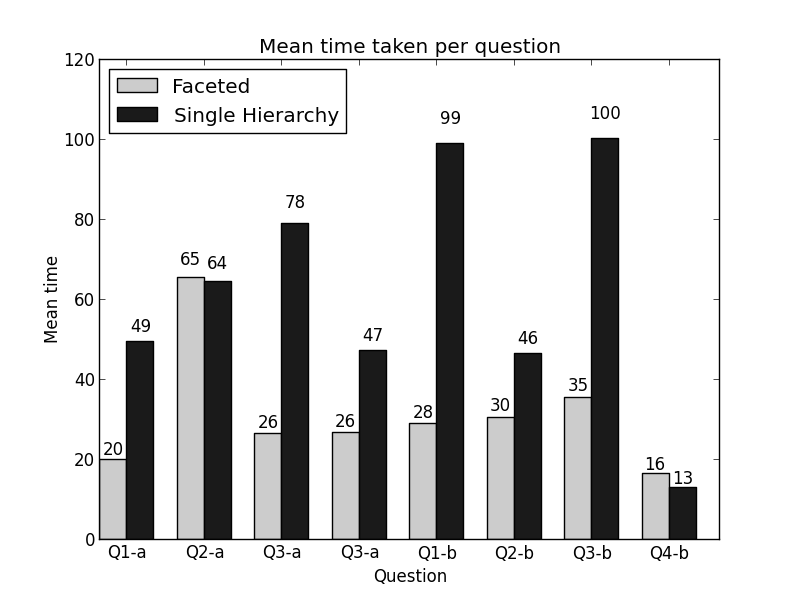
\includegraphics[width=0.5\textwidth]{meantime2.png}
  }
  \subfloat[Ratings for each interface, by user \label{fig:results2}]{
  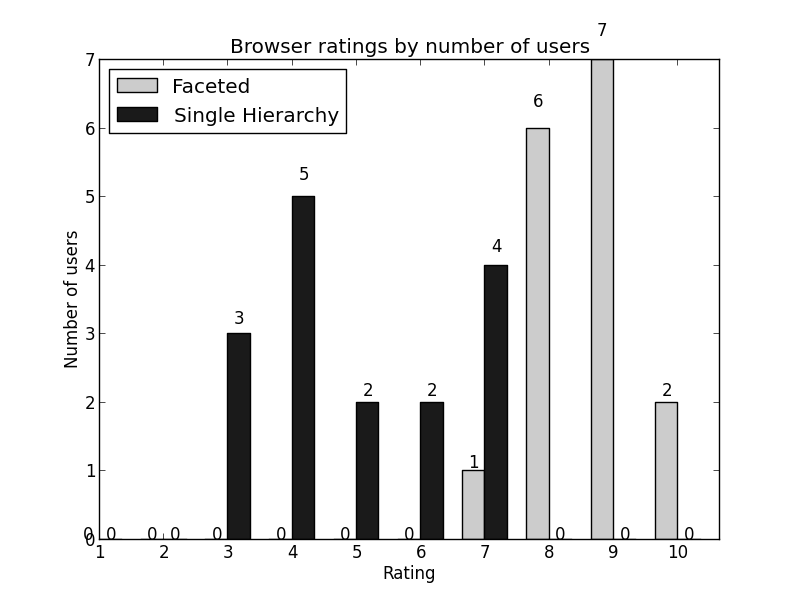
\includegraphics[width=0.5\textwidth]{ratings2.png}
  }
  \label{fig:results}
  \end{figure}
        \begin{itemize}
            \item Faceted vs non-faceted browsers tested
            \item Given tasks to complete and timed
        \end{itemize}
\end{frame}

\begin{frame}
    \frametitle{Conclusions, future work}
        Conclusions:
        \begin{itemize}
            \item Vast majority preferred faceted browser
            \item Faceted was preferred for both task completion and free exploration
        \end{itemize}
        Future work:
        \begin{itemize}
            \item Compare faceted browser with graph visualisation
            \item Genre/medium distinction unclear
            \item Tag names: France vs French. Fuzzy search?
            \item Automatically determine facets
        \end{itemize}
\end{frame}


\begin{frame}
\tiny
    \frametitle{References}
  \begin{thebibliography}{10}    
  \beamertemplatebookbibitems
  \bibitem{sanderson}
  Sanderson, Mark and Croft, Bruce
    \newblock {\em Deriving concept hierarchies from text}.
    \newblock {\em Proceedings of the 22nd annual international ACM SIGIR conference on Research and development in information retrieval}, pg. 206-213, 1999.
  \beamertemplatearticlebibitems
  \bibitem{schmitz}
  Schmitz, Patrick
    \newblock Inducing ontology from flickr tags
    \newblock {\em Collaborative Web Tagging Workshop at WWW2006, Edinburgh, Scotland}, 2006.
  \beamertemplatearticlebibitems
  \bibitem{heymann}
  Heymann, Paul and Garcia-Molina, Hector
    \newblock Collaborative creation of communal hierarchical taxonomies in social tagging systems
    \newblock {\em Stanford Press}, 2006.
  \beamertemplatearticlebibitems
  \bibitem{ranganathan}
  Ranganathan, Shiyali Ramamrita
    \newblock Prolegomena to library classification
    \newblock 1967.
  \beamertemplatearticlebibitems
  \bibitem{hearst}
  Hearst, Marti and Elliott, Ame and English, Jennifer and Sinha, Rashmi and Swearingen, Kirsten and Yee, Ka-Ping
    \newblock Finding the flow in web site search
    \newblock {\em Communications of the ACM}, 45(9):42-49, 2002.
  \end{thebibliography}
\end{frame}

\end{document}
